57. Получить числа 7 и 36 можно только как $7:1=7$ и $4\times9=36.$ Тогда из остальных цифр нужно выбрать два, дающих в сумме третье так, чтобы оставшиеся два числа отличались на 4. Это можно сделать единственным способом.
\begin{center}
\begin{figure}[ht!]
\center{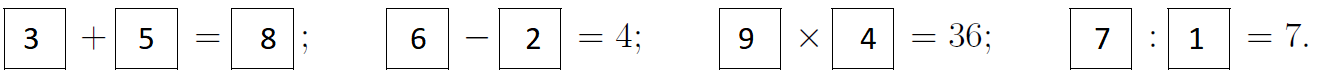
\includegraphics[scale=0.35]{11s.png}}
\end{figure}
\end{center}
